%%%%%
%%%%%  Use LUALATEX, not LATEX.
%%%%%
%%%%
\documentclass[]{VUMIFTemplateClass}

\usepackage{indentfirst}
\usepackage{amsmath, amsthm, amssymb, amsfonts}
\usepackage{mathtools}
\usepackage{physics}
\usepackage{graphicx}
\usepackage{verbatim}
\usepackage[hidelinks]{hyperref}
\usepackage{color,algorithm,algorithmic}
\usepackage[nottoc]{tocbibind}
\usepackage{tocloft}

\usepackage{titlesec}
\newcommand{\sectionbreak}{\clearpage}

\makeatletter
\renewcommand{\fnum@algorithm}{\thealgorithm}
\makeatother
\renewcommand\thealgorithm{\arabic{algorithm} algorithm}

\usepackage{biblatex}
\bibliography{bibliografija}
%% to change the numbering (numeric or alphabetic) of bibliographic sources, make the change in VUMIFTemplateClass.cls, line 139

% Author's MACROS
\newcommand{\EE}{\mathbb{E}\,} % Mean
\newcommand{\ee}{{\mathrm e}}  % nice exponent
\newcommand{\RR}{\mathbb{R}}


\studyprogramme{Software Engineering} %Write your study programme (example – Software engineering, Financial and Actuarial Mathematics, etc.)
% \worktype{\{Work type\}} % Bachelor's thesis or Master's thesis
\worktitle{Team agreement}
% \workauthor{Name Surname}

%There may be more than one author, in which case each author is written from a new line which is added in Titlepage.tex or LongerTitlePage.tex
%\secondauthor{Name Surname} %If present, otherwise delete

% \supervisor{pedagogical/scientific title Name Surname}
\reviewer{Team members} %If present, otherwise delete
% \scientificadvisor{pedagogical/scientific title Name Surname} %If present, otherwise delete

\begin{document}
\selectlanguage{english}

\onehalfspacing
\begin{titlepage}
\vskip 20pt
\begin{center}

\includegraphics[scale=0.55]{images/MIF.png}
\end{center}

\makeatletter

\vskip 20pt
\centerline{\bf \large \textbf{VILNIUS UNIVERSITY}}
\vskip 10pt
\centerline{\large \textbf{FACULTY OF MATHEMATICS AND INFORMATICS}}
\vskip 10pt
\centerline{\large \textbf{\MakeUppercase{\@studyprogramme \space study programme}}}

\vskip 80pt
\centerline{\Large \@worktype}
\vskip 20pt
\begin{center}
    {\bf \LARGE \@worktitle}
\end{center}
\begin{center}
    {\bf \Large \@secondworktitle}
\end{center}
\vskip 80pt

\centering{\Large \@workauthor}
\@ifundefined{@secondauthor}{}
{
\vskip 10pt
\centering{\Large \@secondauthor}
}
\vskip 20pt

\centering{
    \begin{tabular}{rcp{.7\textwidth}}
        {\Large Supervisor} & {\Large :} & {\Large \@supervisor}\\[10pt]
        \@ifundefined{@scientificadvisor}{}
            {
                {\Large Scientific advisor} & {\Large :} & {\Large \@scientificadvisor}\\[10pt]
            }
        \@ifundefined{@reviewer}{}
            {
                {\Large Reviewer} & {\Large :} & {\Large \@reviewer}\\[10pt]
            }
    \end{tabular}}


\vskip 110pt

\centerline{\large \textbf{Vilnius}}
\centerline{\large \textbf{\the\year{}}}

\makeatother

\newpage
\end{titlepage}
%\newgeometry{top=2cm,bottom=2cm,right=2cm,left=3cm}
\setcounter{page}{2}


%% Acknowledgements Section
\sectionnonumnocontent{Acknowledgements}
The author is thankful the Information Technology Research Center, Faculty of Mathematics and Informatics, Vilnius University, for providing the High-Performance Computing (HPC) resources for this research.
%%
%%
%%      If you have used IT resources (CPU-h, GPU-h, other IT resources) provided by MIF for your thesis research, please leave the acknowledgement; if you have not, you can delete it.
%%
%%

You can also add here acknowledgements for various other things, such as your supervisor, university, company, etc.

%%Summary
\sectionnonum{Summary}

Summary in english.\\

\textbf{Keywords:} work related keywords, with a \textit{\textbf{minimum of 3 keywords}}, but can be more.

\sectionnonum{Santrauka}

Darbo santrauka.\\

\textbf{Raktiniai žodžiai:} čia surašomi su darbu susiję raktiniai žodžiai, \textit{\textbf{minimalus raktinių žodžių kiekis - 3}}, tačiau jų gali būti ir daugiau.




\singlespacing
\selectlanguage{english}
% list of figures, delete if not needed
\listoffigures 

%list of tables, delete if not needed
\listoftables

%Turinys
\tableofcontents
\onehalfspacing


%Section for symbols
\sectionnonum{List of symbols} %Leave if necessary
This section is for when symbols are used. For example:
\begin{itemize}
    \item $\EE X$ denotes the mean of the random variable $X$.
\end{itemize}


%Section for abbreviations
\sectionnonum{List of abbreviations} %Leave if necessary
This section is for when abbreviations are used. For example:

\begin{tabular}{rcp{.7\textwidth}}
    {u.d.i.r.v.} & {} & {uniformly distributed independent random variables}
\end{tabular}

\sectionnonum{Introduction}
For any written work, you must refer to the methodology guidelines of the respective study programme\footnote{The latest methodology requirements for all programmes can be found here, in the respective programme: \url{https://mif.vu.lt/lt3/en/studies/bachelor-studies}}. These contain all the guidelines for citations, structure, length, etc.


\section{Formatting}

This section will give you examples of how to format mathematical text, tables and figures, and describe how to correctly formulate the mathematical results of your final thesis.

\subsection{Mathematical text}

Mathematical formulas can be embedded in paragraphs of text by separating the formulas \LaTeX~code with \texttt{\$...\$}. Example: trigonometric identity $\sin^2 \alpha + \cos^2 \alpha = 1$.

However, formulas will look much nicer if they are separated into separate equations by placing the formula code in the environment \texttt{\textbackslash[...\textbackslash]}. Example of an equation:
\[
\ee^{i \alpha} = \cos{\alpha} + i \sin{\alpha}, \qquad \alpha \in \RR.
\]
The mathematical symbols $\RR$ and $\ee$ have been used in this equation, with the commands \texttt{\textbackslash RR} and \texttt{\textbackslash ee} defined at the beginning of this template. Sometimes formulas take several lines, e.g.:
\begin{equation}
\begin{split}
2&= 1+1+0=\left(\frac{\sqrt{16}}{\tan^2\pi/3+1}\right) +\ln\ee+\sin\pi\\
&= (\sin^2 17+\cos^2 17)^{\ln\ee}+\cos 0 +(x^{1/\ln x})'. 
\label{form1}
\end{split}
\end{equation}
Don't forget to put a full stop (.) at the end of the formula if it is the end of a sentence. Also note the height of brackets with a large fraction inside \texttt{\textbackslash frac}, which is automatically adjusted with \texttt{\textbackslash left( ... \textbackslash right)} or specified with \texttt{\textbackslash big}, \texttt{\textbackslash Big}, \texttt{\textbackslash bbig}.

\bigskip

If the formula is needed later, it does not need to be rewritten each time. You can always quote the formula you need with the \texttt{\textbackslash eqref} command. For example, the formula with the number above is quoted as follows: equation \eqref{form1}. To do this, the \texttt{\textbackslash label} command must assign a temporary name to the formula, which \LaTeX~ will automatically change to the required number. More information on \LaTeX~mathematical symbols, equations, mathematical environments and commands can be found in this document \cite{amsdoc}.

\bigskip

Here are some more formulas that use more complex mathematical commands. Matrices and determinants are written using the LaTeX environments \texttt{pmatrix} and \texttt{vmatrix}:
\[
A= \begin{pmatrix}
    0 & 1\\
    2 & 3
\end{pmatrix}, \qquad
\det A =
\begin{vmatrix}
0 & 1\\
2 & 3    
\end{vmatrix} = 0 \cdot 3 - 1 \cdot 2 = -2.
\]
For more complex equations and matrices, the \texttt{mathtools} \cite{mtoolsdoc} commands are very useful. The \texttt{mathtools} package is included in the working template, so you can use its commands directly.

The derivative is written using an apostrophe character (\texttt{'}), for example,
\[
(f(x)g(x))' = f'(x)g(x) + f(x)g'(x).
\]
Taylor polynomial:
\[
p(x) = p(a) + p'(a)(x-a)+\frac{p''(a)}{2!}(x-a)^2 + ... + \frac{p^{(n)}}{n!}(x-a)^n.
\]
For writing simple and partial derivatives, differentials, gradients, etc., the template includes the very handy commands \texttt{\textbackslash dv} and \texttt{\textbackslash pdv}, \texttt{\textbackslash dd}, \texttt{\textbackslash grad} from the \texttt{physics} package \cite{physdoc}:
\[
\dv{f}{x},  \qquad
\dv[2]{f}{x}, \qquad
\pdv{f}{x},  \qquad
\pdv[5]{f}{x} \qquad
\pdv{f}{x}{y}, \qquad
\dd{f}, \qquad
\grad{f}
\]

To write the integral in an interval, use the \LaTeX command \texttt{\textbackslash int\textunderscore \{a\}\^{}\{b\}}:
\[
\int_{a}^{b}f(x) \dd x = F(a) - F(b) = \eval{F(x)}_{a}^{b}
\]
For writing multiple, surface, curvilinear integrals you can use the commands \texttt{\textbackslash iint}, \texttt{\textbackslash iiint}, \texttt{\textbackslash oint}, etc.
\[
\iint_{D}f(x, y)\dd{x}\dd{y},\quad
\iint_{D} f(x,y)\dd{S}, \quad
\int_{\gamma} f(x,y)\dd{l},\quad
\oint_{\gamma} P(x,y)\dd{x}+Q(x,y)\dd{y}.
\]

\subsection{Matematinių rezultatų formulavimas}

To formulate the mathematical results of your work, you should use environments
\[
\text{\emph{Definition}},\qquad \text{\emph{Proposition}}, \qquad \text{\emph{Theorem}}, \qquad \text{\emph{Lemma}},
\]
\[
\text{\emph{Corollary}}, \qquad \text{\emph{Remark}}, \qquad  \text{\emph{Example}}, \qquad \text{\emph{Proof}}.
\]
These environments are already defined
in your thesis template \texttt{VUMIFTemplateClass.cls}, by combining the standard \LaTeX\ commands
\[
\texttt{definition}, \qquad \texttt{proposition}, \qquad \texttt{theorem}, \qquad \texttt{lemma},
\]
\[
\texttt{corollary}, \qquad \texttt{remark}, \qquad \texttt{example}, \qquad \texttt{proof}.
\]
\noindent Example of a definition:
\begin{definition}
A number $p \in \mathbb{N}$ is called a \emph{prime number} if it is divisible only by $1$ and itself. The set of prime numbers is denoted by $\mathbb{P}$.
\end{definition}
\noindent Example of a proposition:
\begin{proposition}
The average of the product of two independent random variables $X, Y: \Omega \to \mathbb{R}$ is equal to the product of the averages of the two original variables $XY$:
\[
\EE{(XY)}=\int_{\Omega} X(\omega)Y(\omega)\dd\mu(\omega) = \EE{X} \cdot \EE{Y},
\]
provided that the means of $X$, $Y$ and $XY$ exist.
\end{proposition}

\noindent  Important mathematical statements are called \emph{theorems}:
\begin{theorem}[First theorem on isomorphism]\label{teor1}
    Suppose that $f: G {\rightarrow} H$ is a homomorphism between the groups G and H. Then the image $f(G)$ of the group $G$ is isomorphic to the factor group $G / \ker{(f)}$, that is
    \[
        f(G) \cong G \big / \ker{(f)}.
    \]
\end{theorem}

\noindent The shorter auxiliary statements are called \emph{lemmas}. However, lemma formulations can also be quite complex:
\begin{lemma}[Vector substitution lemma]\label{lem1}
    Suppose that the vectors of the linear space V over the body k
    \begin{equation}\label{šeima1}
        v_1, v_2, \dots, v_s
    \end{equation}
    are linearly independent, and that each vector $v_i$, $1 \leq i \leq s$ of this family is linearly expressed in vectors
    \begin{equation}\label{šeima2}
        w_1, w_2, \dots, w_t.
    \end{equation}
    Then $s \leq t$, and there exists a subfamily $w_{j_1}, w_{j_2}, . . . , w_{j_s}$ of the vector family \eqref{šeima2}, which we replace by the vectors $v_1, v_2, . . . , v_s$, we get a family of vectors \eqref{šeima2} equivalent to the family \eqref{šeima2}.
\end{lemma}

\noindent The \emph{Remark} environment is for small remarks:

\begin{remark}
The condition of the theorem that the interval $[a, b]$ is compact and the function $f(x)$ is continuous on that interval is essential.
\end{remark}

\noindent Another environment \emph{Example} is used for short numerical or formula examples:

\begin{example}
Systems of equations
\[
\left\{
\begin{array}{rclcl}
    ax & + & by & = & e\\
    cx & + & dy & = & f
\end{array}
\right.
\]
Kramer's formula for solutions:
\[
x = \frac{D_{x}}{D}, \qquad y = \frac{D_{y}}{D},\]
here
\[
D=
\begin{vmatrix}
a & b\\
c & d    
\end{vmatrix}=ad-bc, \qquad
D_x=
\begin{vmatrix}
e & b\\
f & d    
\end{vmatrix}=ed-bf, \qquad
D_y=
\begin{vmatrix}
a & e\\
c & f    
\end{vmatrix}=af-ec.
\]
\end{example}

\noindent The \texttt{proof} syntax is used to record evidence. Below is a proposition and a proof of that proposition. The end of the proof is automatically marked with the \square\ symbol by \LaTeX.
\begin{proposition}
  A square matrix $A$ is non-singular if and only if $\det A \ne 0$.
\end{proposition}
\begin{proof}
    If $A$ is non-singular, then there exists a matrix $B$ such that $AB=I$. By the determinant property of the product of matrices,
    \[
        \det A \cdot \det B = \det AB = \det I = 1.
    \]
    Therefore, $\det A \ne 0$.
    Now suppose that $\det A \ne 0$. Let $A^*$ be a transposed adjoint matrix. Then:
     \[\begin{split}
        A A^* =
        \begin{pmatrix}
            a_{11} & \dots & a_{1n} \\
            \vdots & \ddots & \vdots \\
            a_{n1} & \dots & a_{nn} \\
        \end{pmatrix} \cdot
        \begin{pmatrix}
            A_{11} & \dots & A_{n1} \\
            \vdots & \ddots & \vdots \\
            A_{1n} & \dots & A_{nn} \\
        \end{pmatrix} 
&=  \begin{pmatrix}
            \det A  & \dots & 0 \\
                  0 & \ddots & 0 \\
                  0 & \dots & \det A \\
        \end{pmatrix}
        \\
        &=\det A \cdot
        \begin{pmatrix}
            1 & \dots & 0\\
            0 & \ddots & 0\\
            0 & \dots & 1
        \end{pmatrix} = \det A \cdot I.
    \end{split}\]

    So, $A \cdot A^* = \det A \cdot I$. Dividing both sides of the identity by the $\det A \ne 0$ gives $A \cdot \left(\frac{1}{\det A}A^*\right) = I$. Similarly, we can show that $\left(\frac{1}{\det A}A^*\right) \cdot A = I$. Hence, $\frac{1}{\det A}A^*$ is the inverse of the matrix $A$, and hence $A$ is non-singular.
    \end{proof}

    \bigskip

    Please note that mathematical environments are numbered automatically. Like formulas, mathematical definitions, statements, examples can be cited elsewhere in the text by first naming them with \texttt{\textbackslash label} and then creating a citation reference \texttt{\textbackslash ref} at the appropriate place. For example, we can quote Theorem \ref{teor1} or Lem \ref{lem1} in the places in the text where we need to refer to them.

\subsection{Tables}

If tables are presented, the table references should be mentioned in the text, for example: the \ref{tab:xydata} table shows some results.

\begin{table}[H]
    \centering
    \caption{Tables are numbered at the top, caption is at the top}
    \begin{tabular}{|c|c|c|}
        \hline
        Column 1 & Column 2 & Column 3 \\
        \hline
         & &  \\
         \hline
         & & \\
         \hline
    \end{tabular}
    \label{tab:xydata}
\end{table}


Each table must have a title, which, like the table number, must appear on the same line above the table. All tables shall be numbered consecutively (letter numbering is not recommended, e.g. Table 7a).

\subsection{Images, graphs, charts, photos}
If figures are used in the work, they must be mentioned in the text, e.g.:~\ref{fig:graph1}~ figure shows an example of how to present a figure.

\begin{figure}[H]
    \centering
    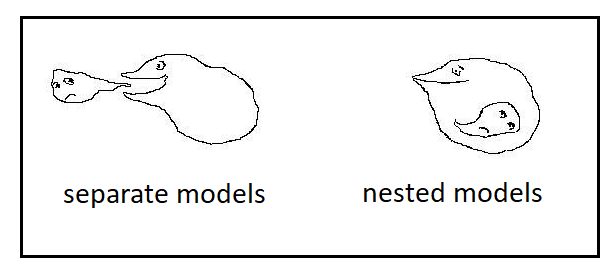
\includegraphics[width=0.5\textwidth]{images/AIC.png}
    \caption{Figure numbers are at the bottom, caption is at the bottom}
    \label{fig:graph1}
\end{figure}


Below is the text after the image.

\subsection{Lists}

Example of a non-numbered list:
\begin{itemize}
    \item first element;
    \item second element.
\end{itemize}

Example of a numbered lists:
\begin{enumerate}
    \item lorem ipsum dolor sit amet;
    \item consectetur adipiscing elit;
    \item vivamus a nisl gravida.
\end{enumerate}


\section{Presentation of software code}
This section outlines the way in which software code can be presented.

\subsection{Algorithms}

Algorithms are numbered in the same way as figures or tables. They must be mentioned in the text, e.g.:~\ref{alg:gd} is used to find the minimum value of the function $\mathcal{L}$.

\begin{algorithm}[h]
\caption{Gradual descent pseudocode}\label{alg:gd}
\begin{algorithmic}[1]
    \STATE \textcolor{blue}{\texttt{\textbf{\# We assume that $\mathcal{L}$ is defined in the text}}}
        \STATE Input: $\mathcal{D}$ -- dataset
        \STATE Input: $\theta_0$ -- initializing random values for parameters
        \STATE Input: $\gamma$ -- learning rate, step size
        \STATE Input: $m$ -- number of epochs
        \FOR{$i = 1, 2, \dots, m$}
            \STATE $\theta_i \coloneq \theta_{i-1} - \gamma \nabla_\theta \mathcal{L}(\mathcal{D}, \theta_{i-1})$
            \STATE \textcolor{blue}{\texttt{\textbf{\# The derivative of function $\mathcal{L}$ is calculated automatically by autograd}}}
        \ENDFOR
\end{algorithmic}
\end{algorithm}

\subsubsection{Subsubsection example}
\noindent No need to use lots of \textit{subsubsections}.

\sectionnonum{Results and conclusions}
For details of what needs to be written in this section, please refer to the methodology requirements of the respective programme. 

\printbibliography[title = {References and sources}]


\appendix
\renewcommand{\thesection}{Appendix \arabic{section}. }

\section{\phantom{Appendix} Examples of citations}
In the document \textit{bibliography.bib}, you need to add all the cited sources and after using the function \textit{\{\textbackslash cite\{name of the cited object\}\}} the corresponding source will be added to the list of literature sources.


\textit{bibliography.bib} provides examples of some of the most commonly cited types of sources:
\begin{itemize}
    \item web pages (\textit{@online}) \cite{PvzInternetinisPuslapis},
    \item datasets (\textit{@dataset}) \cite{dataset}
    \item articles (\textit{@article}) \cite{PvzStraipsnLt, PvzStraipsnEn}, 
    \item articles from conferences (\textit{@inproceedings}) \cite{PvzKonfLt, PvzKonfEn}, 
    \item books (\textit{@book}) \cite{PvzKnygLt, PvzKnygEn}, 
    \item theses (\textit{@thesis or mastersthesis/phdthesis} \cite{PvzMagistrLt, PvzPhdEn})
    \item electronic publications (\textit{@misc}) \cite{PvzElPubLt, PvzElPubEn}
\end{itemize}

Examples are also provided for ChatGPT citation, both in general \cite{chatgpt_bendrai} and for a specific conversation \cite{chatgpt_pokalbis}.

\end{document}
